%%%%%%%%%%%%%%%%%%%%%%%%%%%%%%%%%%%%%%%%%%%%%%%%%%%%%%%%%%%%
% Document settings
\documentclass{ACGSeminar}

%%%%%%%%%%%%%%%%%%%%%%%%%%%%%%%%%%%%%%%%%%%%%%%%%%%%%%%%%%%%
% Own Packages

%%%%%%%%%%%%%%%%%%%%%%%%%%%%%%%%%%%%%%%%%%%%%%%%%%%%%%%%%%%%
% Own Definitions
\newcommand{\comment}[1]{}


%%%%%%%%%%%%%%%%%%%%%%%%%%%%%%%%%%%%%%%%%%%%%%%%%%%%%%%%%%%%
% BibTex
\bibliography{references}

%%%%%%%%%%%%%%%%%%%%%%%%%%%%%
% Hyphenations here
%%%%%%%%%%%%%%%%%%%%%%%%%%%%%
\hyphenation{Sa-tan-arch-aeo-li-deal-co-hell-ish}


%%%%%%%%%%%%%%%%%%%%%%%%%%%%%
% Title, Author, etc.

\begin{document}

\title{Re: Deep G-Buffers for Stable Global Illumination Approximation}

\author{Ferit Tohidi Far}

\maketitle

%%%%%%%%%%%%%%%%%%%%%%%%%%%%%%%%%%%%%%%%%%%%%%%%%%%%%%%%%%%%
% Abstract

\begin{abstract}%
G-buffers can be used to efficiently render images with large amounts of light sources. This is possible thanks to a process called "deferred rendering". Using 
g-buffers, we are only able to compute local illumination. By using deep g-buffers instead we can approximate global illumination, which is way more 
efficient than traditional global illumination methods like pathtracing, while of course not being physically accurate. 
\end{abstract}

\keywords{g-buffer, deep g-buffer, pathtracing, global illumination, deferred shading, deferred rendering}
\tableofcontents

\label{cha:references}

\newpage

%%%%%%%%%%%%%%%%%%%%%%%%%%%%%%%%%%%%%%%%%%%%%%%%%%%%%%%%%%%%
% Introduction
\label{cha:introduction}
\section{Global Illumination}
	Global Illumination is a lighting effect that is achieved by not only computing direct light, but also indirect light, meaning that it is neccesary to take
	into account how light reflects and carries information (in the most basic case: color).
	\subsection{Physically correct methods}
	In order to generate physically correct images, which is a requirement for creating photorealistic images, we need to solve the rendering equation
	$$ L_o(\omega) = L_e(\omega) + \int_\Omega f(\omega, \omega')L_i(\omega')cos(n, \omega') \partial \omega' $$
	where 
	\begin{center}
		\begin{align*}
			&L_o(\omega) \text{ is the outgoing light in direction } \omega\text{,}\\
			&L_e(\omega) \text{ is the emmited light in direction } \omega\text{,}\\
			&f(\omega, \omega') \text{ is the BRDF} \footnote{BRDF (Bidirectional random distribution function) returns the reflection direction (and refraction?) of a surface.} \text{,}\\
			&L_i(\omega') \text{ is the incoming light from direction } \omega'\\
			&\text{and } cos(n, \omega') \text{ is lambert reflectance} \footnote{Lambert reflectance computes the attentuation of light based on its incident angle to the surface.} \text{ .}
		\end{align*}
	\end{center}
	The most popular method for achieving this is pathtracing \cite{P2PATH}.
	\subsubsection{Pathtracing}
		Pathtracing solves the rendering equation by 
	\subsection{Computational difficulties of physically correct methods}
	Since we have to take into account every ray of light and its reflections, the computational difficulty becomes apparent \cite{DST}.
	% TODO insert time-complexity of pathtracing and time-complexity of deferred-rendering for comparison

\section{Deferred Rendering}
	\subsection{How deferred rendering handles lighting more efficiently}
		The goal of deferred rendering is to postpone the shading stage. %TODO insert information about graphics pipeline of gpu
		Instead of shading right away, we compute necessary geometry buffers (g-buffers) and cache 
		them for later use. For all practical purposes, g-buffers have to at least consist of a frame-buffer, a normal-buffer and a z-buffer. Using only these g-buffers, 
		we can now compute the shading separately.
	\subsection{Deferred Shading}

\section{Geometry-buffer (g-buffer)}
	Each geometry-buffer stores information of some sort for each individual pixel, meaning that they are all two-dimensional arrays.
	\subsection{Frame-Buffer}%
		The frame-buffer stores color values.% 
		\begin{figure}[htb!]%
			\begin{center}%
				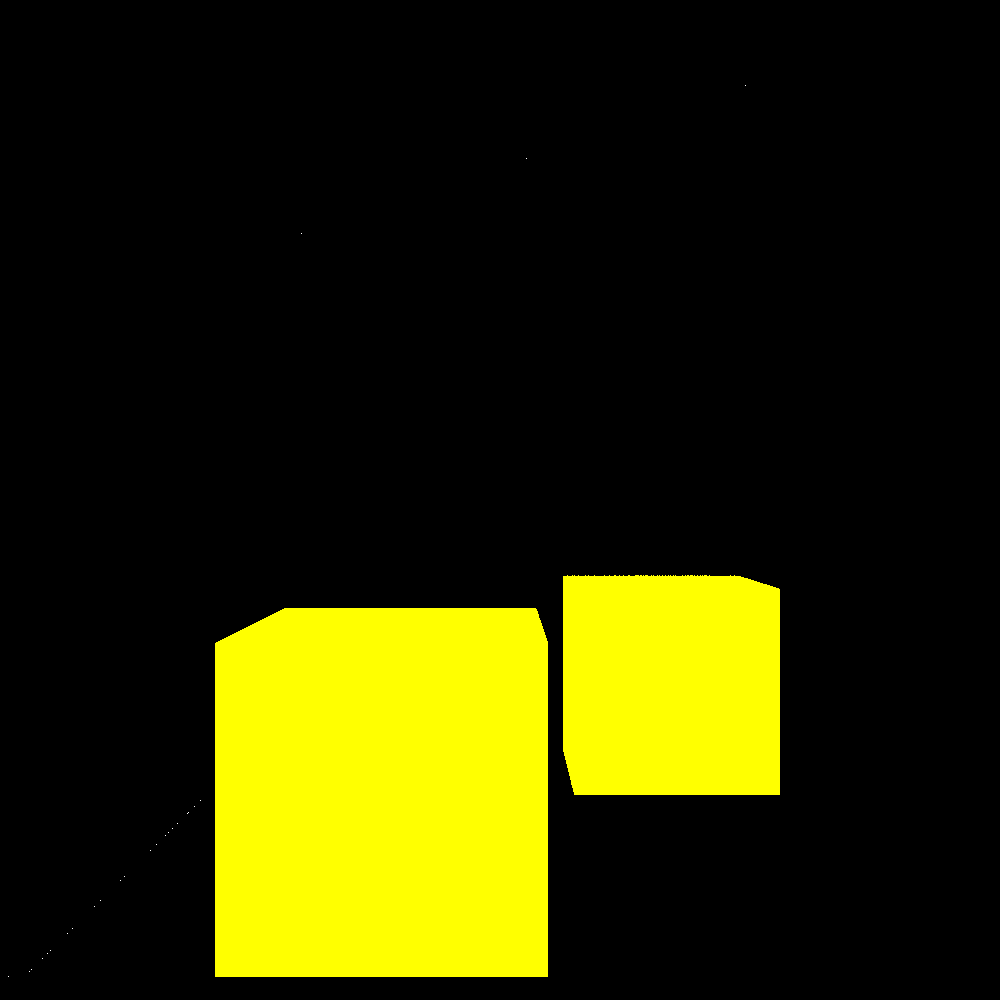
\includegraphics[width=6cm]{img/frame_buffer.png}
			\end{center}%
			\caption{Example of a frame-buffer (also called image-buffer)}%
			\label{fig:frame_buffer}%
		\end{figure}%
	\subsection{Z-Buffer}
		The z-buffer stores depth values.
		\begin{figure}[htb!]%
			\begin{center}%
				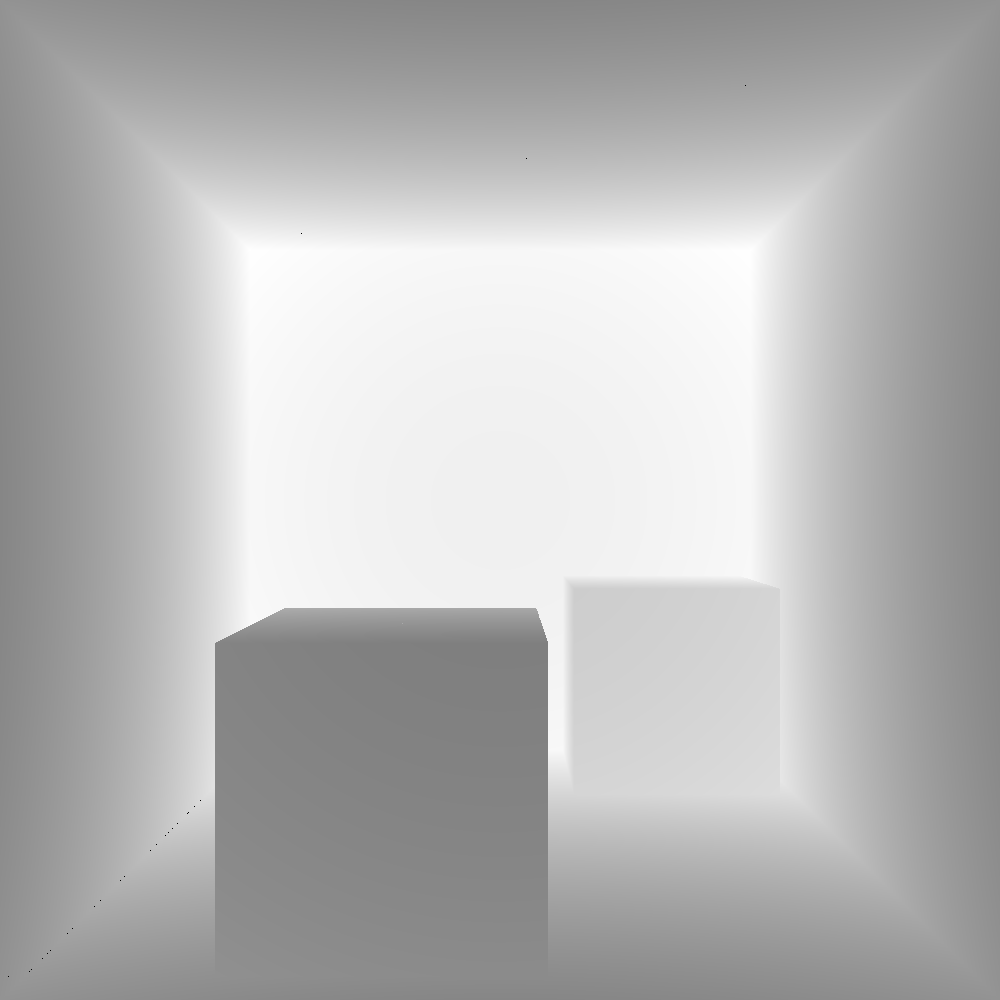
\includegraphics[width=6cm]{img/z_buffer.png}
			\end{center}%
			\caption{Example of a z-buffer}%
			\label{fig:z_buffer}%
		\end{figure}%
	\subsection{Normal-Buffer}
		The normal-buffer stores surface-normals.
		\begin{figure}[htb!]%
			\begin{center}%
				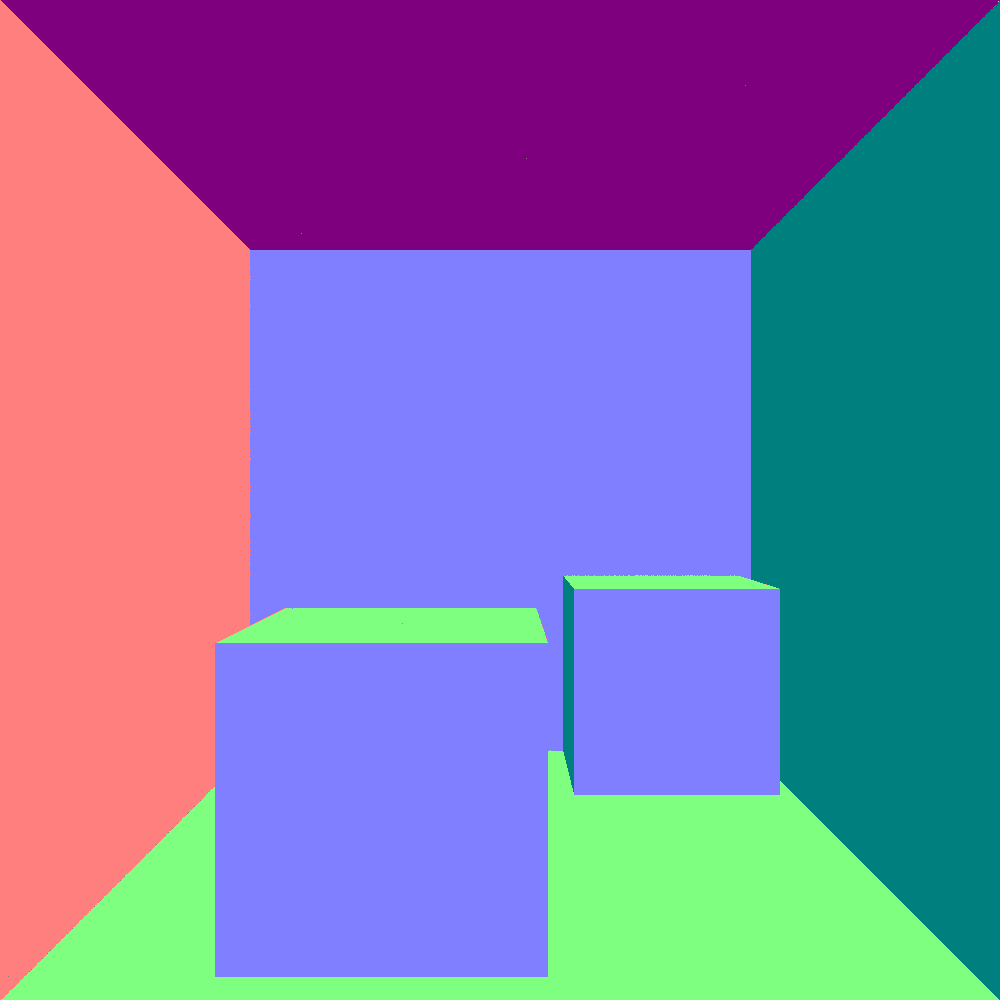
\includegraphics[width=6cm]{img/normal_buffer.png}
			\end{center}%
			\caption{Example of a normal-buffer}%
			\label{fig:normal_buffer}%
		\end{figure}%
		Note that there are more possible buffers to choose from, but the three that were mentioned are the most essential in every g-buffer.
	\subsection{Computing local illumination using g-buffers}
		After collecting all g-buffers we can now work on illumination. To do this we need to define some light sources. We distinguish between three types of lights:
		Point-lights, spot-lights and directional-lights \cite{DST}.

\section{Deep G-Buffer}
	\subsection{Concept}
		Deep g-buffers use a concept similar to depth peeling. Instead of storing information about the closest surface, we also store information about the n-closest surface (n layer deep g-buffer). \cite{NDGB}.
	\subsection{How Deep G-Buffers approximate visual effects}


\section{Visual effects}
	The following are visual effects that are sought after, but hard/impossible to achieve physically correct without using
	computationally expensive methods. When using pathtracing, we get all of the following effects for free: 
	\subsection{Ambient occlusion}
		Ambient occlusion essentially describes how much shading the "in-betweens" of a 3d object gets. This effect can be efficiently approximated by using a method called - ironically - screen space ambient occlusion (SSAO). This method basically runs an edge detector over the z-buffer and paints those edges black. Since it only runs over the z-buffer it is considered screen space.
		%TODO insert graphics for AO here
	\subsection{Color bleeding}
		Color bleeding happens when light directs information from one hit-surface to another. Let A and B be objects. If A reflects light onto B and A's surface is blue, then B will also appear
		to be slightly blue on the reflected area. To have this happen it is obviously necessary to trace rays of some sort. This can be approximated, though, using ... %TODO how is this approximated?
		%TODO insert graphics for color bleeding here
	\subsection{Soft shadows}
		We can easily compute hard shadows using shadow mapping. This is done by projecting the scene from the light source's point of view and then projecting the scene from the camera's point of view while only actually painting the points with their respective colors if they were visible, else they are painted black. To get soft shadows, the points in shadow simply get blended together with their surrounding points.
		%TODO insert graphics for soft and hard shadow
	\subsection{Transparency}
		A quick method to achieve transparency is depth peeling. \cite{NOIT}.

	\subsection{Reflection}
		Reflection ...

\section{Performance and Output Comparison}
	\subsection{Deep G-Buffers vs Pathtracing}

%%%%%%%%%%%%%%%%%%%%%%%%%%%%%%%%%%%%%%%%%%%%%%%%%%%%%%%%%%%%
% Bibliography
\printbibliography

\end{document}
